\documentclass[conference]{IEEEtran}
%\IEEEoverridecommandlockouts
% The preceding line is only needed to identify funding in the first footnote. If that is unneeded, please comment it out.
% Template version as of 6/27/2024

\usepackage{cite}
\usepackage[ngerman]{babel}
\usepackage{amsmath,amssymb,amsfonts}
\usepackage{algorithmic}
\usepackage{graphicx}
\usepackage{textcomp}
\usepackage{listings}
\usepackage[utf8]{inputenc}
\usepackage[justification=centering]{caption} % Paket für Captions
\usepackage{xcolor}
\usepackage{url}
%\usepackage{todonotes}
\newcommand{\todo}[1]{\textcolor{red}{TODO: #1}}
\def\BibTeX{{\rm B\kern-.05em{\sc i\kern-.025em b}\kern-.08em
    T\kern-.1667em\lower.7ex\hbox{E}\kern-.125emX}}
\begin{document}

\lstset{
    basicstyle=\normalfont\footnotesize,
    keywordstyle=\bfseries, % Nur fett, keine Farbe
    stringstyle=\color{violet},
    commentstyle=\color{green!70!black},
    showstringspaces=false,
    numbers=none,
    breaklines=true,
    captionpos=b,
}

\title{FPGAs in DBMS
}

\author{\IEEEauthorblockN{1\textsuperscript{st} Felix Grenzing}
    \IEEEauthorblockA{\textit{Universität Hamburg} \\
        Hamburg, Deutschland\\
        felix.grenzing@studium.uni-hamburg.de}
}

\maketitle

\begin{abstract}
    Abstract here.
\end{abstract}

\begin{IEEEkeywords}
    FPGAs, DBMS, Hardware Acceleration
\end{IEEEkeywords}

\section{Einführung}


\section{Begriffe}
In~\cite{li_bitweaving_2013} und~\cite{lisa_column_2018} werden verschidene Begriffe verwendet, die Erklärung bedürfen.


\subsection{FPGAs}


\subsection{Einsatzmöglichkeiten}

FPGAs können in Datenbanksystemen auf verschiedene Weisen eingesetzt werden. Klassischer Weise gibt es On-the-Side Beschleuniger, wobei die CPU die Daten
besitzt und der FPGA über eine Schnittstelle wie PCIe angebunden ist. Die CPU muss in diesem Szenario die Daten an den FPGA senden und die Ergebnisse wieder
empfangen. Diese Architektur wurde häufig auch mit GPUs umgesetzt.

Eine andere Möglichkeit ist die In Datapath Beschleunigung, bei der der FPGA direkt in den Datenpfad eingebunden ist. Der FPGA kann die Daten in Echtzeit
verarbeiten und die Ergebnisse mit gleicher Geschwindigkeit an die CPU zurückgeben. Häufig ist das Ziel die Datenmenge zu reduzieren, da nahe der
Datenquelle häufig höhere Bandbreiten zur Verfügung stehen. Die Architektur ist somit mit Smart-Storage Lösungen verwandt.

Eine dritte Möglichkeit ist die Koprozessor Architektur, bei der der FPGA als Koprozessor der CPU fungiert. Der FPGA ist auf demselben Chip wie die CPU
und hat häufig auch direkten Speicherzugriff. Flaschenhälse durch langsame Schnittstellen können so vermieden werden, was Vorteile gegenüber
\mbox{On-the-Side} Beschleunigern bietet.



% \begin{figure}[htbp]
%     \centering
%     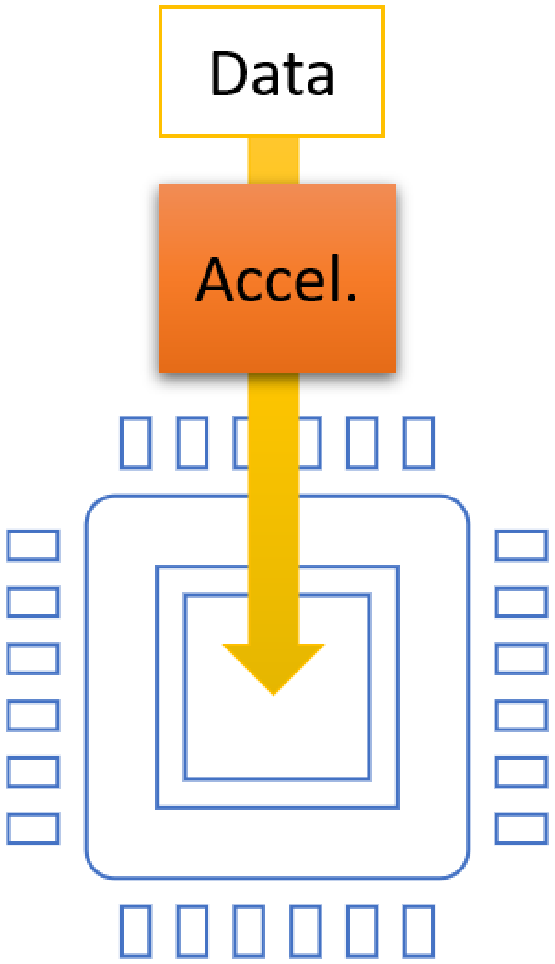
\includegraphics[width=0.1\textwidth]{imgs/InDatapath.png}
%     \caption{In Datapath Architektur}
%     \label{fig:indatapath}
% \end{figure}

% \begin{figure}[htbp]
%     \centering
%     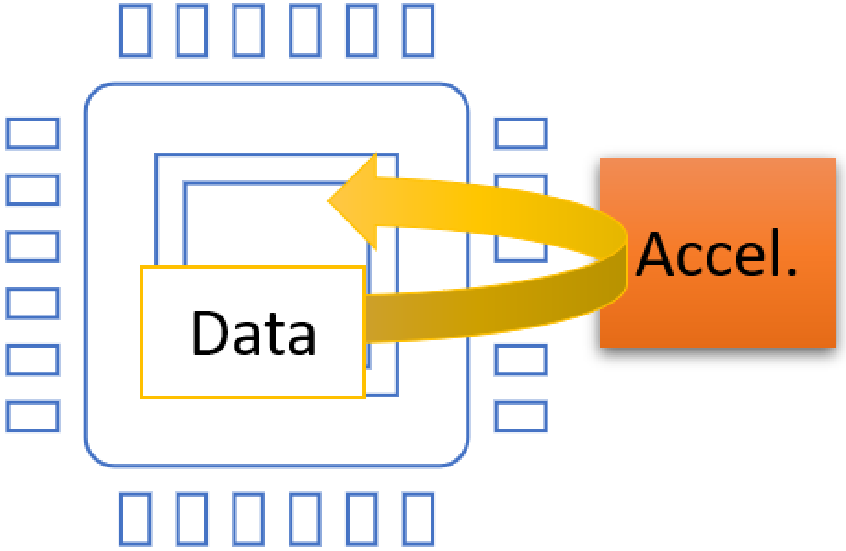
\includegraphics[width=0.15\textwidth]{imgs/OnTheSide.png}
%     \caption{On The Side Architektur}
%     \label{fig:ontheside}
% \end{figure}


% \begin{figure}[htbp]
%     \centering
%     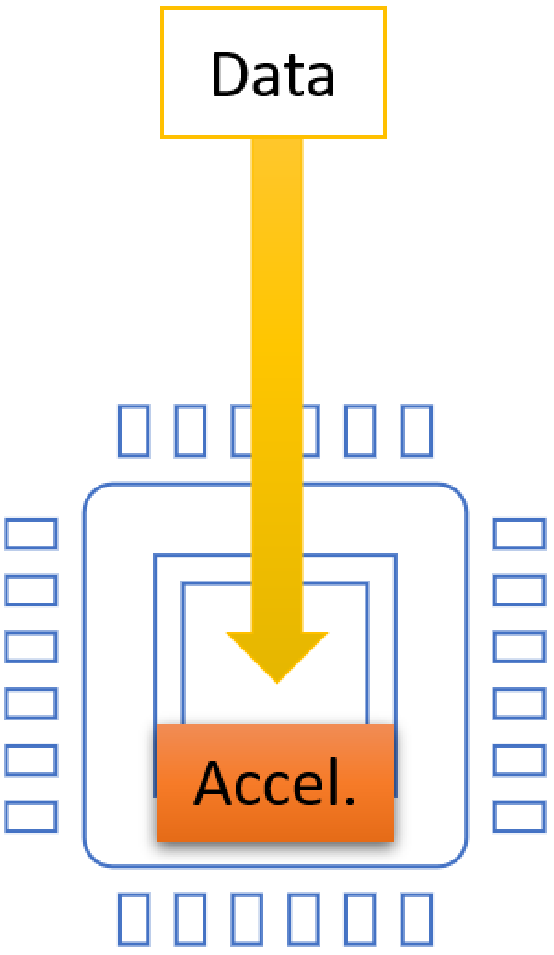
\includegraphics[width=0.1\textwidth]{imgs/Coprocessor.png}
%     \caption{Koprozessor Architektur}
%     \label{fig:coprocessor}
% \end{figure}

\subsection{Pipelining und Datenparallelität}
Zwei wichtige Arten der Parallelität sind die Pipelineparallelität und die Datenparallelität. Pipelineparalleität beschreibt die Aufteilung der Befehlsabarbeitung
in mehrere Stufen, die parallel arbeiten. Jede Stufe bearbeitet dabei Teil des Befehls und gibt die Ergebnisse an die nächste Stufe weiter.
Ein Beispiel für eine Pipeline ist in Abbildung~\ref{fig:pipeline} zu sehen. Die Befehle werden in vier Stufen aufgeteilt. Bearbeitet die Fetch Stufe den ersten Befehl.
Sobald dies geschehen ist, wird der Befehl an die nächste Stufe weitergegeben. Die Fetch Stufe kann nun den nächsten Befehl bearbeiten. Die Befehle werden so stufenweise
durch die Pipeline geschoben.

\begin{figure}[htbp]
    \centering
    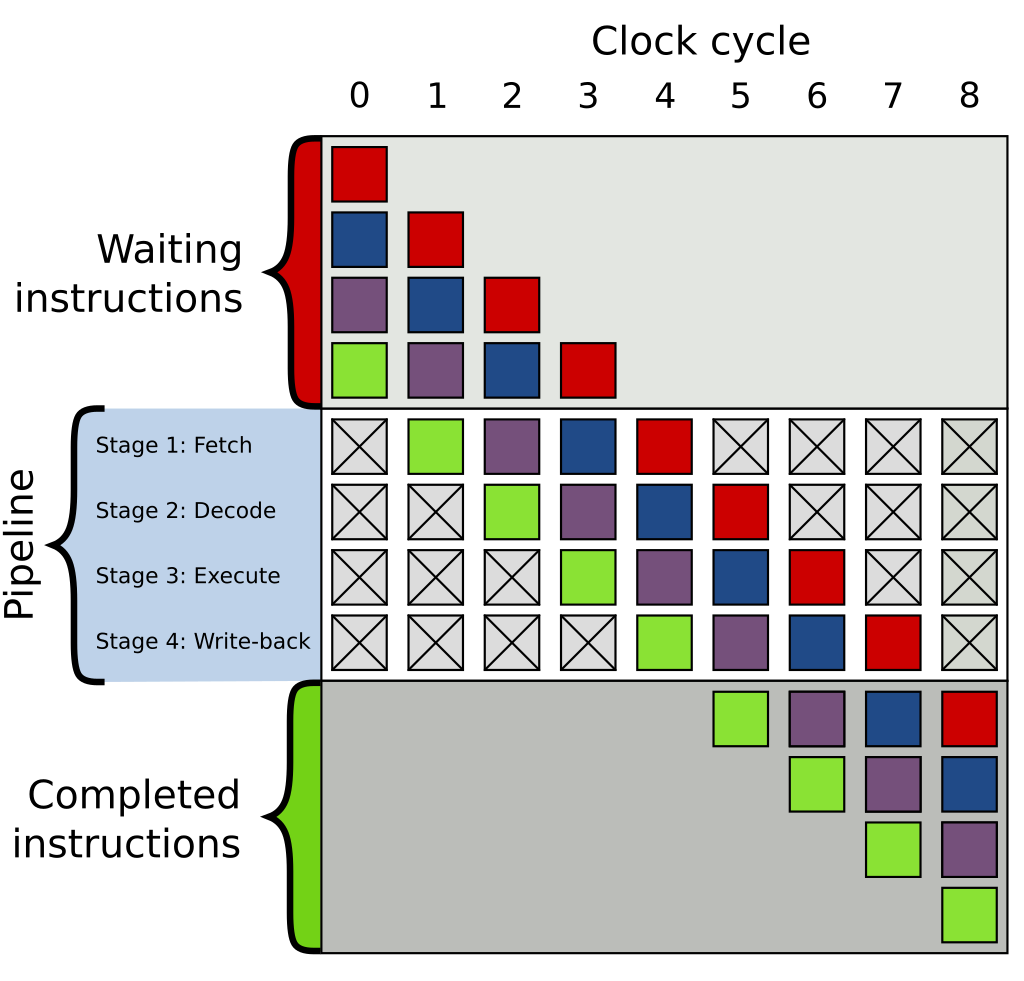
\includegraphics[width=0.25\textwidth]{imgs/pipeline.png}
    \caption{Prozessor Pipeline~\cite{wikipedia_pipeline}}
    \label{fig:pipeline }
\end{figure}

Datenparallelität beschreibt die Aufteilung der Daten in mehrere Teile, die mit mehreren Bearbeitungseinheiten parallel verarbeitet werden. Beide Ansätze können die Performance
von Algorithmen verbessern, und können auch kombiniert werden um die Vorteile beider Ansätze zu nutzen. Um beide Ansätze zu kombinieren, könnten mehrere Pipelines entworfen werden,
die jeweils verschidene Datenbearbeiten.



\subsection{Partial Reconfiguration}
Partial Reconfiguration (PR) ist ein Konzept, welches aktuelle FPGAs unterstützen. PR bietet die Möglichkeit, Teile des FPGAs zur Laufzeit zu verändern,
ohne das gesamte FPGA neu zu konfigurieren oder das FPGA offline nehmen zu müssen. Dies ermöglicht es, verschiedene Funktionen auf einem FPGA zu implementieren
und bei Bedarf zu wechseln. Umkonfiguration während der Laufzeit bietet offensichtlich Pozenzial für Beschleunigung, da mehr Algorithmen implementiert
werden können, als gleichzeitig auf dem FPGA Platz haben. Eine Problematik ist jedoch, dass die Umkonfiguration Zeit in Größenordnungen von Millisekunden benötigt.

Das Projekt DoppioDB~\cite{li_bitweaving_2013} nutzt PR, um verschiedene Algorithmen auf einem FPGA zu implementieren und bei Bedarf zu wechseln.

\subsection{BitWeaving}
\todo{Faktcheck}
BitWeaving ist ein Algorithmus, der in~\cite{li_bitweaving_2013} vorgestellt wird. Der Algorithmus stellt eine Methode dar, Spaltenscanoperationen durchzuführen, indem
die Daten mehrerer Zeilen als Bitvektor codiert in einem Prozessorwort gespeichert und verarbeitet werden. Zwei Varianten des Algorithmus werden vorgestellt, BitWeaving H und BitWeaving V,
die sich in der Art und Weise unterscheiden, wie die Daten in den Prozessorworten gespeichert werden. BitWeaving H speichert die Daten zeilenweise, BitWeaving V spaltenweise.


\section{Einordnung der Situation}
Die Rolle von FPGAs in Datenbanksystemen ist laut \cite{istvan_glass_2019} aktuell einem Wandel unterzogen. Während bei FPGAs in der Vergangenheit
Herausforderungen die Potenziale überwogen haben, bieten aktuelle Entwicklungen neue Möglichkeiten für den Einsatz von FPGAs in Datenbanksystemen.

~\cite{istvan_glass_2019} stellt diese Entwicklung als Gegensätze von Pessimismus der Vergangenheit und Optimismus der Gegenwart und Zukunft dar.

\subsection{Pessimismus}
Der Pessimismus der Vergangenheit begründete sich fundamental in drei Probelemen.

Erstens war die Anbindung der On-the-Side Beschleuniger an die CPU ein Flaschenhals, da die Kommunikation in beiden Richtungen über
einen Bus erfoglen musste, welcher zu hohe Latenzen und zu geringe Bandbreiten bot. \todo{Quelle} On-the-Side Beschleuniger waren
die gängige Architektur, um Datenbankoperationen zu beschleunigen, welche nicht im Datenpfad durchgeführt werden können.
Koprozessor Architekturen wurden von Chipherstellern nicht wirklich angeboten und waren somit nicht weit verbreitet.

Zweitens profitieren nicht alle Algorithmen von der Beschleunigung durch FPGAs. Iterative Algorithmen, die auf den Ergebnissen vorheriger
Iterationen aufbauen, können nicht von der hohen Parallelität von FPGAs profitieren. \todo{Quelle} CPUs sind in diesen Fällen performanter,
da die hohen Taktraten die itertiven Instruktionen abarbeiten können. Auch weit verzweigte Algorithmen, mit vielen If-Else Anweisungen
sind nicht für FPGAs geeignet, da jeder Pfad im FPGA implementiert werden muss, was zu hohen Ressourcenverbrauch führt. Hoher Ressourcenverbrauch
wiederrum führt zu geringerer Parallelität, da weniger paralelle Pipelines implementiert werden können. Die Inkompatibilität von Algorithmen
wird durch den ersten Punkt noch verstärkt, da die schwierige Kommunikation zwischen CPU und FPGA die Entwickler dazu zwingt, gesamte Algorithmen
auf dem FPGA zu implementieren, anstatt nur die Teile, die von der Beschleunigung profitieren, um die Kommunikation zu minimieren.

Drittens ist die direkte Konkurrenz von CPUs ein Hinderniss. CPUs sind sehr flexible, sie können theoretisch jeden Algorithmus
ausführen. Hinzu kommt, dass die Leistung der CPUs stetig steigt (Moores's Law) und die Taktraten immer höher werden. Durch den hohe
Zeit- und Ressourcenaufwand, welcher die Entwicklung von FPGA Beschleunigern mit sich bringt, war es häufig nicht praktikabel, FPGAs
anstelle von CPUs für Datenbankbeschleunigung zu nutzen.

\subsection{Optimismus}
Der Optimismus für die Gegenwart und Zukunft, den der Autor motiviert, basiert auf drei wesentlichen Entwicklungen.

Erstens haben sich die Architekturen verändert. Moderne FPGAs sind häufig als Koprozessoren direkt auf dem gleichen Chip wie die CPU integriert,
was die Latenzen und Bandbreitenprobleme der On-the-Side Beschleuniger, durch direkten Speicherzugriff des FPGAs, löst. \todo{Quelle}
Diese enge Integration ermöglicht granulare Beschleunigung, bei der nur die Teile des Algorithmus, die von der Beschleunigung profitieren,
auf dem FPGA implementiert werden. Die erhöhte Verfügbarkeit von Koprozessor Architekturen bestärkt nun auch die Erforschung und Entwicklung
von FPGA Beschleunigern was zu einer Vielzahl von neuen Anwendungen führt (siehe~\cite{lisa_column_2018},~\cite{sidler_accelerating_2017}).


Zweitens haben sich die Workloads verändert. Bisher wurden hauptsächlich klassische SQL-Operatoren in Datenbank durchgeführt, welche auf der verfügbaren Hardware
häufig Memory-bound waren, also durch die Geschwindigkeit der Datentransfers limitiert. Durch neue Anwendungen wie Maschinelles Lernen und Künstliche Intelligenz
sind neue Workloads entstanden, die häufig Compute-bound sind, also durch die Geschwindigkeit der Berechnungen limitiert. Da diese Anwendungen viele Daten benötigen,
liegt es nahe, die Anwendungen als neue Daatenbank Operatoren einzuführen. Für Compute-bound Workloads werden FPGAs wieder interessant, da sie durch ihre
hohe Parallelität und Rekonfigurierbarkeit die Berechnungen beschleunigen können.

Drittens ermöglichen hybride Ansätze eine bessere Nutzung der Stärken von FPGAs und CPUs. Durch die Kombination beider Technologien
können Algorithmen so aufgeteilt werden, dass die parallelisierbaren Teile auf dem FPGA und die sequentiellen Teile auf der CPU ausgeführt werden. Ein Beispiel dafür ist
REGEXP\_LIKE~\cite{sidler_accelerating_2017}.
\todo{Quelle}


\section{Anderes Paper} % BitWeaving
Im Kontext veränderter Architekturen ordnet sich auch~\cite{lisa_column_2018} ein. Dort wurde auf einem FPGA ein Column Store implementiert, der
den BitWeaving H Algorithmus nutzt. Es wurden verschidenen Hardwareansätze verglichen, um die beste Performance zu erzielen.

\subsection{Architektur}
Die Forschung von~\cite{lisa_column_2018} baut auf der Zynq Ultrascale+ Architektur von Xilinx auf. Die Plattform ist aus zweiteilig aus Steuersystem mit
4 ARM Cortex-A53 Kernen und 4GB DDR4 Speicher und Logikbereich mit FPGA und 500MB DDR4 Speicher aufgebaut~\cite{lisa_column_2018}.
\todo{Mehr}

\subsection{Grundlegendes Vorgehen}
Pipeline

Processing Elements

Combiner



\subsection{Verschiedene Ansätze}

Mehrere paralelle Pipelines -> Datenparallelität

Limitation des DDR4-Controlers

Optimale Nutzung von Combiner

Hybridansatz



\subsection{Ergebnisse}

\section{Andere Ansätze}

\subsection{IBEX}
IBEX ist ein FPGA-basierter Beschleuniger für Datenbanken, der in~\cite{istvan_glass_2019} vorgestellt wird. IBEX ist ein In-Data-Path Beschleuniger,
der direkt in den Datenpfad eingebunden ist, also zwischen SSD und der CPU. Die Daten werden mit gleicher Bandbreite verarbeitet, wie sie von der SSD
ankommen. Der FPGA führt SQL-Operatoren aus, welche die Datenmenge reduzieren, also beispielsweise Filter und Aggregationen, nicht aber Operatoren,
die die Datenmenge erhöhen können, wie Joins. IBEX verwendet auch einen hybriden Ansatz, um Aggregate zu berechnen. Die Aggregatfunktionen werden auf dem FPGA
mit einem Hashtable berechnet, welcher mit fester Größe im RAM verortet ist, was gleiche Laufzeiten, unabhängig von den Daten ermöglicht, da der Hashtable nicht
dynamisch vergrößert werden muss, aber dadurch die Anazhl der Gruppen bei Aggregatbildung limitiert. Um dieses Limit zu umgehen, gibt der FPGA Teilaggregate
weiter, sobald der Hashtable keinen Platz mehr für neue Gruppen hat. Die CPU vereinigt dann die Teilaggregate zu einem Endergebnis auf eine Weise, das die Bearbeitung
von der Arbeit des FPGAs in jedem Fall profitiert. Der FPGA kann so die Datenmenge reduzieren und die CPU kann die reduzierte Datenmenge effizienter verarbeiten.

\subsection{Caribou}

\subsection{DoppioDB}
Das Projekt DoppioDB zeigt einen solchen Ansatz, indem die Datenbank die FPGA-Steuerung
übernimmt und Hardware-Threads nutzt, die wie Software-Threads angesprochen werden. Dabei wurde über SQL hinausgehend Funktionalität für maschinelles Lernen integriert, wie z. B.
stochastische Gradientenabstiege und Entscheidungsbaum-Inferenz.
\todo{FIXME}

\subsection{REGEXP\_LIKE}
Ein vorgestelltes Projekt befasst sich mit der Optimierung des REGEX\_LIKE Operators, welcher reguläre Ausdrücke auf Datenbanken anwendet. So können beispielsweise
alle Zeilen einer Tabelle selektiert werden, die in einer Spalte einen bestimmten regulären Ausdruck erfüllen. Der Operator wurde auf einem FPGA implementiert
und zeigt die Nutzung von hybriden Ansätzen, indem die relevanten Daten so weit wie möglich auf dem FPGA verarbeitet werden und nur falls nötig auf der CPU
nachbearbeitet werden~\cite{sidler_accelerating_2017}. So können alle REGEXP\_LIKE-Anfragen durch die Beschleunigung profitieren, da nicht vollständig passende
reguläre Ausdrücke nicht abgewiesen und damit vollständig auf der CPU verarbeitet werden müssen.

Der Reguläre Ausdruck wird an an einer Wildcard-Position aufgeteil, so dass zwei unabhängige reguläre Ausdrücke entstehen. Der FPGA gibt dann, zusammen mit einem Index
alle Zeilen zurück, die den ersten regulären Audruck erfüllen. Die CPU überprüft dann, ob die Zeilen vom Index aus auch den zweiten regulären Ausdruck erfüllen.
Der verwendete Ausdruck in~\cite{sidler_accelerating_2017} ist in Listing~\ref{lst:regexp} zu sehen. Der FPGA bearbeitet den Ausdruck bis zur zweiten
Wildcard und die CPU muss dann nur noch nach `delivery' suchen.


\begin{lstlisting}[language=SQL,frame=single,caption={Regulärer Ausdruck aus \cite{sidler_accelerating_2017}},label={lst:regexp}]
SELECT count(*) 
FROM address_tables
WHERE REGEXP_LIKE(address_string,
'(Strasse|Str\.).*(8[0-9]{4}).*delivery');
\end{lstlisting}

\section{The Road that lies ahead}
Ein zentraler Aspekt der zukünftigen Datenbankentwicklung ist die Integration programmierbarer Hardware wie FPGAs, die zwar neu konfigurierbar, jedoch nicht so flexibel wie Software sind.
Die Kernfrage hierbei ist, wer die Kontrolle über die Beschleunigungsfunktionen übernimmt -- das Betriebssystem bzw. der Hypervisor oder die Datenbank selbst.

\subsection{Betriebssystem- oder Datenbankverwaltung?}

Wenn das Betriebssystem die Kontrolle behält, muss die Datenbank Strategien entwickeln, um von hardwarebasierten Beschleunigungsmöglichkeiten zu profitieren,
die vom Infrastruktur- oder Cloudanbieter bereitgestellt werden. Hierbei könnten bereits etablierte Techniken zur Code-Optimierung für spezifische CPU-Features,
wie SIMD-Einheiten, als Grundlage dienen.

Übernimmt hingegen die Datenbank die Kontrolle, eröffnen sich größere Gestaltungsspielräume. Die Datenbank könnte benutzerdefinierte Hardware-Beschleuniger entwickeln,
die exakt auf ihre Bedürfnisse abgestimmt sind, und diese sogar zur Laufzeit synthetisieren (Siehe DoppioDB)
% Zukünftige Forschungsfragen umfassen, wie eine Bibliothek hardwarebasierter Operatoren aufgebaut und welche Granularität diese Operatoren haben sollten,
% um maximale Effizienz zu erreichen. Herausforderungen der Hardware-Programmierung

% FIX 
% Eine weitere wichtige Fragestellung betrifft die effiziente Ausdrucksweise für Hardware-Beschleuniger im Kontext von Datenbanken. Während CPUs und GPUs feste Architekturen besitzen, ist dies bei FPGAs nicht der Fall, was zusätzliche Komplexität bei der Planung und Kompilierung von Abfragen mit sich bringt. Moderne Ansätze, wie die Entwicklung domänenspezifischer Sprachen (DSLs) für Hardware-Beschleuniger, könnten diesen Prozess erleichtern.

% Eine mögliche Richtung ist die Verwendung von Ansätzen wie der Spatial-Sprache, die die physische Anordnung von Schaltkreisen berücksichtigt. Solche DSLs könnten als Zwischenschritt zwischen SQL und Hardware dienen, um Sub-Operator-Pipelines automatisch auf FPGAs auszulagern.

% Die Übersetzung von Datenbank-Operatoren auf Hardware bleibt jedoch schwierig, insbesondere da Hardware-Ressourcen oft begrenzt sind. Dies erfordert hybride Ansätze, bei denen Corner Cases durch Software nachbearbeitet werden, ohne die Gesamtleistung zu beeinträchtigen. Die Automatisierung geeigneter Aufteilungspunkte zwischen Hardware- und Software-Funktionalitäten ist dabei eine offene Herausforderung.

% Dieser Abschnitt zeigt, dass die Integration programmierbarer Hardware eine Balance zwischen Flexibilität und Leistung erfordert, wobei sowohl Datenbankentwickler als auch Hardware-Designer neue Ansätze und Lösungen erarbeiten müssen.

\bibliographystyle{IEEEtran}
\bibliography{FPGAs}

\end{document}
